\section{Preprocessing Data (Tiền xử lý dữ liệu)}

\subsection{Giới thiệu chung về vai trò của tiền xử lý dữ liệu trong khai thác dữ liệu}

\hspace{0.5cm}Trong dự án này, tiền xử lý dữ liệu đóng vai trò quan trọng trong việc chuẩn bị dữ liệu về chất lượng không khí cho mô hình học máy. Dữ liệu thô (\textit{raw data}) chứa thông tin về các chỉ số ô nhiễm không khí, nhiệt độ, độ ẩm và thời gian, cần được xử lý để đảm bảo tính chính xác và hiệu quả của mô hình dự đoán.

\begin{figure}[h]
    \centering
    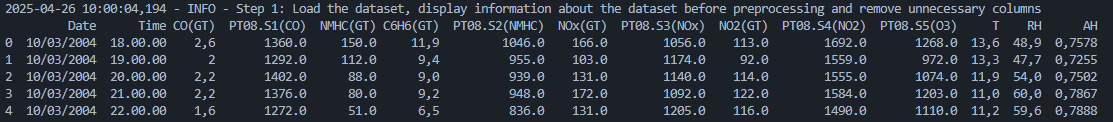
\includegraphics[width=0.9\textwidth]{images/raw_data_preview.png}
    \caption{Hiển thị dữ liệu gốc trước khi tiền xử lý}
    \label{fig:raw_data_preview}
\end{figure}

\begin{figure}[h]
    \centering
    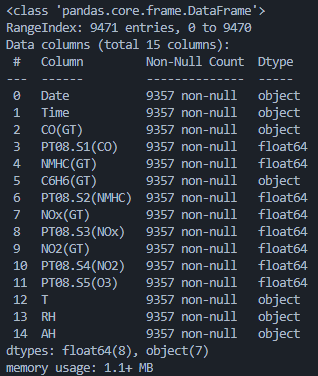
\includegraphics[width=0.9\textwidth]{images/raw_data_statistics.png}
    \caption{Thống kê mô tả dữ liệu gốc}
    \label{fig:raw_data_statistics}
\end{figure}

\subsection{Quá trình tiền xử lý dữ liệu}

\subsubsection{Bước 1: Xử lý các cột không cần thiết}
\hspace{0.5cm}Đầu tiên, nhóm loại bỏ các cột không cần thiết như "Unnamed: 15" và "Unnamed: 16" để làm sạch dữ liệu.

\subsubsection{Bước 2: Xử lý giá trị thiếu}
\hspace{0.5cm}Đối với các cột số học, giá trị thiếu được thay thế bằng giá trị trung bình của cột đó. Đối với các cột dạng chuỗi, giá trị thiếu được thay thế bằng giá trị xuất hiện thường xuyên nhất.

\subsubsection{Bước 3: Chuyển đổi kiểu dữ liệu}
\hspace{0.5cm}Các cột dữ liệu được chuyển đổi sang kiểu dữ liệu phù hợp:
\begin{itemize}
    \item Cột "Date" được chuyển đổi từ định dạng DD/MM/YYYY sang datetime
    \item Cột "Time" được chuyển đổi từ định dạng HH.MM.SS sang time
    \item Các cột số học được chuẩn hóa bằng cách thay thế dấu phẩy bằng dấu chấm
    \item Cột CO(GT) có giá trị -200 được thay thế bằng giá trị trung bình
\end{itemize}

\subsubsection{Bước 4: Xử lý ngoại lệ (outliers)}
\hspace{0.5cm}Nhóm sử dụng phương pháp Z-score để xác định và xử lý các giá trị ngoại lệ:
\begin{itemize}
    \item Tính toán Z-score cho mỗi cột số học
    \item Xác định ngưỡng là 3 độ lệch chuẩn
    \item Thay thế các giá trị ngoại lệ bằng giá trị trung bình của cột
    \item Đặc biệt xử lý cột NMHC(GT) để đảm bảo không có giá trị âm
\end{itemize}

\begin{figure}[h]
    \centering
    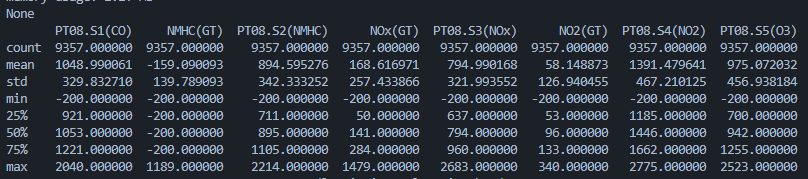
\includegraphics[width=0.9\textwidth]{images/data_distribution_comparison.png}
    \caption{So sánh phân phối dữ liệu trước và sau khi xử lý ngoại lệ}
    \label{fig:data_distribution}
\end{figure}

\subsubsection{Bước 5: Tạo đặc trưng mới}
\hspace{0.5cm}Nhóm tạo các đặc trưng mới từ dữ liệu hiện có:
\begin{itemize}
    \item Kết hợp cột "Date" và "Time" thành cột "Date\_Time"
    \item Trích xuất thông tin năm, tháng, ngày và giờ từ cột "Date\_Time"
    \item Tạo các đặc trưng tương tác như Temp\_Humidity, NOx\_NO2
    \item Thêm các đặc trưng thống kê như rolling mean và rolling std
\end{itemize}

\subsection{Kết quả tiền xử lý dữ liệu}

\subsubsection{Thông tin tổng quan về dữ liệu}
\hspace{0.5cm}Sau khi tiền xử lý, bộ dữ liệu có các đặc điểm sau:
\begin{itemize}
    \item Số lượng mẫu: 9,471
    \item Số lượng đặc trưng: 18
    \item Các kiểu dữ liệu:
    \begin{itemize}
        \item float64: 13 cột
        \item datetime64[ns]: 1 cột
        \item int32: 4 cột
    \end{itemize}
\end{itemize}

\begin{figure}[h]
    \centering
    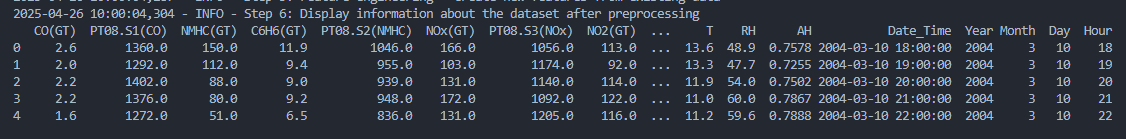
\includegraphics[width=0.9\textwidth]{images/processed_data_preview.png}
    \caption{Hiển thị dữ liệu sau khi tiền xử lý}
    \label{fig:processed_data_preview}
\end{figure}

\subsubsection{Thống kê mô tả}
\hspace{0.5cm}Các thống kê chính của dữ liệu sau tiền xử lý:
\begin{itemize}
    \item CO(GT): Giá trị trung bình 0.77, dao động từ -5.12 đến 11.90
    \item PT08.S1(CO): Giá trị trung bình 1097.15, dao động từ 647 đến 2008
    \item NMHC(GT): Giá trị trung bình 213.58, dao động từ 29 đến 405
    \item C6H6(GT): Giá trị trung bình 10.06, dao động từ 0.10 đến 63.70
\end{itemize}

\begin{figure}[h]
    \centering
    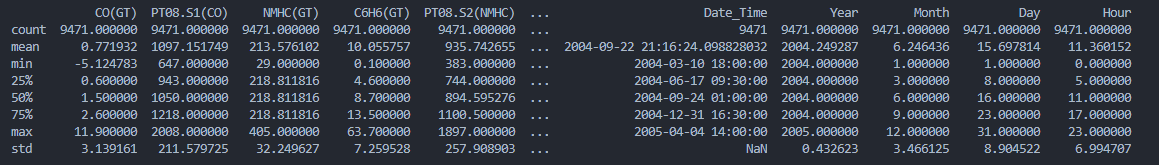
\includegraphics[width=0.9\textwidth]{images/processed_data_statistics.png}
    \caption{Thống kê mô tả dữ liệu sau tiền xử lý}
    \label{fig:processed_data_statistics}
\end{figure}

\subsection{Ý nghĩa của các đặc trưng}

\begin{description}
    \item[CO(GT)]: Nồng độ Carbon Monoxide trong không khí
    \item[PT08.S1(CO)]: Giá trị cảm biến CO
    \item[NMHC(GT)]: Nồng độ Non-methane Hydrocarbons
    \item[C6H6(GT)]: Nồng độ Benzene
    \item[PT08.S2(NMHC)]: Giá trị cảm biến NMHC
    \item[NOx(GT)]: Nồng độ Nitrogen Oxides
    \item[PT08.S3(NOx)]: Giá trị cảm biến NOx
    \item[NO2(GT)]: Nồng độ Nitrogen Dioxide
    \item[PT08.S4(NO2)]: Giá trị cảm biến NO2
    \item[PT08.S5(O3)]: Giá trị cảm biến Ozone
    \item[T]: Nhiệt độ
    \item[RH]: Độ ẩm tương đối
    \item[AH]: Độ ẩm tuyệt đối
    \item[Date\_Time]: Thời gian đo đạc
    \item[Year, Month, Day, Hour]: Các đặc trưng thời gian
\end{description}

\subsection{Kết luận}
\hspace{0.5cm}Quá trình tiền xử lý dữ liệu đã giúp chuẩn bị bộ dữ liệu chất lượng không khí cho việc xây dựng mô hình học máy. Các bước xử lý đã giải quyết các vấn đề về giá trị thiếu, ngoại lệ và tạo thêm các đặc trưng có ý nghĩa. Kết quả cho thấy dữ liệu đã được chuẩn hóa và sẵn sàng cho việc huấn luyện mô hình.